\documentclass[11pt,a4paper,table]{article}

\usepackage{booktabs}
\usepackage[table]{xcolor}
\usepackage[nohyperref]{acl2018} % references acl2018.sty
\usepackage{rotating}
\usepackage{times}
\usepackage{latexsym}
\usepackage{multirow}
\usepackage{graphicx}
	\graphicspath{ {../../plots/} }
\usepackage{url}

\aclfinalcopy % Uncomment this line to show the author and remove the line numbers on the sides

\newcommand{\tabitem}{~~\llap{\textbullet}~~}
\newcommand\BibTeX{B{\sc ib}\TeX}

\title{Optimal Model Input for Newspaper Topic Classification}

\author{Carmen Easterwood \\
  W266 Natural Language Processing with Deep Learning \\
  Summer 2018 \\
}

\date{August 10, 2018}

%%%%%%%%%%%%%%%
% End header information
%%%%%%%%%%%%%%%

\begin{document}
\maketitle

\begin{abstract}
Topic classification is an important method of organizing text content and making it more easily searchable, but in the newspaper setting the question remains: what exactly should we be feeding into topic classification models? In this paper, I test five different model inputs: full text, lead paragraph, headline, nouns-only version of the full text, and lemmatized full text. In general I find that inputs with more words perform better, but that a larger vocabulary isn't necessarily better. While nouns make up only 27\% of the words and 61\% of the vocabulary in a newspaper article, they perform almost as well as the full text, making them possibly the most efficient model input.
\end{abstract}

\section{Introduction}
\label{sec:intro}

Topic classification is an important form of content analysis that has been widely studied in the NLP community. Tagging documents by topic makes searches more efficient, so users can find the information they're looking for more quickly and without having to sort through unrelated documents. Unfortunately, manual topic-coding on a large scale is quite time-consuming, so automating this process can save both time and money for organizations with a large amount of text data.

In this paper, I will look at topic classification specifically in the newspaper context. In addition to making searches more efficient for news consumers and researchers, classifying news articles by topic also helps us understand what journalists are writing about, whether that is changing over time, and the relative importance of different topics. Since many news organizations have seen declining revenue over the last decade \cite{Pew}, a cost-saving measure like automation of topic-coding would likely be welcome. However, in the existing literature there is no agreement on what specifically should be fed into topic classification models to get the best results. In this paper, I develop three supervised topic classification models and test several possible model inputs drawn from New York Times articles. For each model, my main focus is how the model inputs perform relative to each other, and which input gives the best result in each setting.

\section{Background}
\label{sec:back}

As mentioned, there is a large literature looking at topic classification in many contexts, but only a few papers have focused on classifying newspaper articles. Most recently, \citet{Martin:15} found that using a nouns-only or lemmatized version of the articles improved topic classification on a dataset of 90,000 articles from the San Jose Mercury News. However, they were working on an unsupervised model, so they were also relying on the model to generate the topics from the words it received. \citeauthor{Martin:15} evaluated their model using techniques that are not applicable in a supervised setting, so their results are not directly comparable to mine.

Previously, \citet{Wermter:02} proposed a semi-supervised self-organizing memory (SOM) model for topic classification on 100,000 Reuters news articles. The authors were able to achieve accuracies around 90\% for both full text articles and article headlines, and for the full text articles they were able to bump the accuracy up to ~95\% by using WordNet relationships to assist the model (which limited the model input to only the nouns and verbs found in WordNet). Crucially, however, the authors only tested their model on the eight most common topics in their dataset and did not consider articles from other topics. To be useful outside of an academic setting, a topic classification model needs to be able to handle more different types of articles.

Other recent papers have looked at supervised topic classification for non-news documents in various settings. \citet{Karan:16} discusses classification of Croatian political texts using logistic regression (one-vs-rest), Gaussian Naive Bayes, and gradient-boosted trees, as well as utilizing some post-processing rules, to reach an F1 score of 77\% on 22 topics. Their model included lemmas and bigrams as inputs. Meanwhile \citet{Glavas:17} looks at similar political texts in multiple languages, and finds that CNNs perform best for monolingual English models with an accuracy of 57\%. In this paper, I will extend some of the techniques used in these cited works to the news article setting.

\section{Methods}
\label{sec:methods}

\subsection{Dataset}
\label{ssec:dataset}

For this analysis I used the New York Times Annotated Corpus, which contains 1.8 million articles from 1987-2007, labeled with topics, subtopics, and newspaper sections. Due to computing power limitations, I have selected a random sample of 100,000 articles to parse and use as data for the model. The articles are randomly split so that approximately 75\% are training data, 5\% are development data, and 20\% test data.

\subsection{Model Input}
\label{ssec:input}

I test the article's full text and four additional model inputs. Three are pulled from my review of the literature,  and I have added the fourth based on my understanding of the structure of news articles.

\begin{enumerate}
\item \textbf{Full text} of article
\item Article's \textbf{lead paragraph}, which is supposed to hook the reader, and in a news context often summarizes important details of the story \cite{NPR}
\item Article's \textbf{headline} \cite{Wermter:02}
\item \textbf{Nouns-only} version of the full text \cite{Martin:15}. Created using NLTK's part-of-speech tagger.
\item \textbf{Lemmatized} version of the full text \cite{Martin:15}. Created using NLTK's lemmatizer.
\end{enumerate}

Table~\ref{tbl:inputs} shows some key statistics for each type of model input. The full text for the training articles (approximately 75,000 articles) adds up to about 50 million words and a vocabulary of over 300,000 words. The lemmas have roughly the same number of words, but much fewer unique words, with a vocabulary size only 72\% of the full text vocabulary. Then there is a big drop down to the nouns, which have only 27\% of the total words that full text articles have, but 61\% of the vocabulary. As expected, headlines are the smallest category with less than a million words total, and the average individual headline having 8 words.

\begin{table}
	\centering
	\small
	%\makebox[\linewidth]{
	%\resizebox{\columnwidth}{!}{
	\begin{tabular}{lrrr}
		\toprule
		\multirow{2}{*}{\textbf{Model Input}} & \multicolumn{3}{c}{\textbf{Training Words}} \\
		\cmidrule{2-4}
		& \textbf{Count} & \textbf{\% Full Text} & \textbf{Average} \\
		\midrule
		Full Text			& 49.5M	& 100\%	& 668 \\
		Lead Paragraph	& 7.6M	& 15\%	& 105 \\
		Headlines			& 0.6M	& 1\%	& 8 \\
		Nouns			& 13.2M	& 27\%	& 178 \\
		Lemmas			& 50.4M	& 102\%	& 682 \\
		\bottomrule
	\end{tabular}
	\begin{tabular}{lrrr}
		\toprule
		\multirow{2}{*}{\textbf{Model Input}} & \multicolumn{3}{c}{\textbf{Training Vocab (Unique Words)}} \\
		\cmidrule{2-4}
		& \textbf{Count} & \textbf{\% Full Text} & \textbf{Average} \\
		\midrule
		Full Text			& 327K	& 100\%	& 276 \\
		Lead Paragraph	& 140K	& 43\%	& 67 \\
		Headlines			& 42K	& 13\%	& 7 \\
		Nouns			& 198K	& 61\%	& 111 \\
		Lemmas			& 237K	& 72\%	& 253 \\
		\bottomrule
	\end{tabular}
	%}
	\caption{Model Inputs}
	\label{tbl:inputs}
\end{table}

\subsection{Model Output}
\label{ssec:output}

The NYT corpus has multiple ways of classifying articles. Table~\ref{tbl:output} shows four examples from the data of the four different ways the articles were classified. In my models I use the \texttt{desk} column as my model output variable for two reasons:

\begin{enumerate}
\item It has the lowest percentage of null values (0.4\%)
\item It never assigns multiple descriptions to the same article
\end{enumerate}

\begin{sidewaystable*}
\centering
%\small
%\makebox[\linewidth]{
%\resizebox{\columnwidth}{!}{
%\rotatebox{270}{
\begin{tabular}{cllll}
	\toprule
	\textbf{\#} & \textbf{Desk} & \textbf{General Descriptor} & \textbf{Online Sections} & \textbf{Taxonomic Classifier} \\
	\midrule
	1 & Foreign Desk & \tabitem Immigration and Refugees & \tabitem World & \tabitem Top/News/World/Europe \\
	& & \tabitem Jews & & \tabitem Top/News/World/Countries and Territories/Austria \\
	& & \tabitem Music & & \tabitem Top/Features/Arts/Music \\
	& & \tabitem Religion and Churches & & \tabitem Etc. (8 others) \\
	\midrule
	2 & Book Review Desk & \tabitem Books \& Literature & \tabitem Arts & \tabitem Top/Features/Arts \\
	& & & \tabitem Books & \tabitem Top/Features/Books \\
	& & & & \tabitem Top/Features/Books/Book Reviews \\
	\midrule
	3 & Classified & & \tabitem Paid Death Notices & \tabitem Top/Classifieds/Paid Death Notices \\
	\midrule
	4 & Style Desk & \tabitem Computers and the Internet & \tabitem Technology & \tabitem Top/News/Technology \\
	& & \tabitem Labor & \tabitem Style & \tabitem Top/Features/Style/Fashion and Style \\
	& & & \tabitem Opinion & \tabitem Top/Opinion/Opinion \\
	& & & & \tabitem Etc. (2 others) \\
	\bottomrule
\end{tabular}
%}
\caption{Possible Model Outputs}
\label{tbl:output}
\end{sidewaystable*}

However, \texttt{desk} still requires some clean-up before use due to misspellings and possible changes to the desk names over time. Table~\ref{tbl:label-clean} shows some examples of how I cleaned the \texttt{desk} variable so the model would have a standardized set of output labels for the articles. For example, there are significant clusters of articles around "Business/Financial Desk", "Financial Desk", and "Money and Business/Financial Desk" (plus misspellings of each of these), and these are all converted to have a single label of "business \& financial".

\begin{table}
\centering
%\small
\resizebox{\columnwidth}{!}{
\begin{tabular}{clr}
	\toprule
	\textbf{Clean Label} & \textbf{Original Label} & \textbf{Count} \\
	\midrule
	\multirow{2}{*}{book review} & Book Review Desk & 1,750 \\
	& Book Review Dest & 1 \\
	\midrule
	& Business Desk & 4 \\
	& Business World Magazine & 8 \\
	& Business/Financial Desk & 6,078 \\
	& Business/Financial Desk; & 1 \\
	& Business/Financial desk & 1 \\
	& Business/FinancialDesk & 5 \\
	& Business\textbackslash Financial Desk & 2 \\
	business & E-Business & 6 \\
	\& & E-Commerce & 17 \\
	financial & Financial Desk & 11,276 \\
	& Financial Desk; & 16 \\
	& Money \& Business/Financial Desk & 3 \\
	& Money and Busines/Financial Desk & 1 \\
	& Money and Business/Financial Desk & 939 \\
	& Moneyand Business/Financial Desk & 1 \\
	& Small Business & 12 \\
	& SundayBusiness & 82 \\
	& The Business of Green & 3 \\
	\midrule
	\multirow{2}{*}{cars} & Automobiles & 122 \\
	& Cars & 28 \\
	\bottomrule
\end{tabular}
}
\caption{Label Cleaning Examples}
\label{tbl:label-clean}
\end{table}

After label cleaning, roughly 95\% of articles fall into the top 20 categories, and then there are a large number of very small categories with just a few articles. I therefore created an \texttt{<OTHER>} category as a catchall for these tiny categories, which individually don't have enough data for the models to learn very well. Figure~\ref{fig:topnhist} shows the frequency distribution of the top 20 category labels, plus \texttt{<OTHER>}. The top 8-10 categories are "usual suspects" for newspaper sections (e.g. business, sports, classifieds, editorials), and then we see some smaller categories like book reviews and a couple of weekly sections that are unique to the New York Times (New Jersey weekly, the city weekly, Westchester weekly, Long Island weekly).

\begin{figure}
\centering
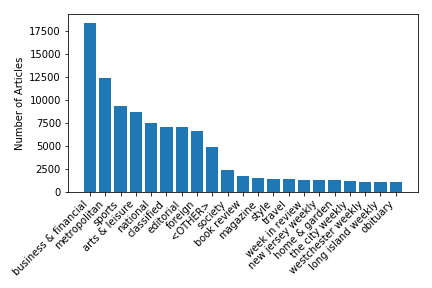
\includegraphics[scale=0.55]{top_n_labels_histogram}
\caption{Frequency of Top 20 Labels + \small{\tt <OTHER>}}
\label{fig:topnhist}
\end{figure}

\subsection{Models}
\label{sec:models}

For each model input, I tested two simple baseline models and a neural network:

\begin{enumerate}
\item Multinomial na\"{i}ve Bayes
\item Multi-class logistic regression (one vs. rest)
\item Convolutional neural network
\end{enumerate}

\subsubsection{MNB and LR}
\label{sssec:mnb-lr}

For the multinomial naive Bayes and logistic regression models, I TF-IDF vectorized the model input, dropping any words with a document frequency count of one. This significantly reduced the vocabulary sizes and got rid of a lot of misspellings and one-off words that just added extra noise to the models.

In each of these models I tested multiple parameter values on the dev data, and chose the parameter values that resulted in the highest accuracy. Figures~\ref{fig:mnb-acc} and~\ref{fig:lr-acc} show how the models performed with different parameter values, and reveal some interesting comparisons between the five model inputs that I will discuss further in Section~\ref{sec:results}.

\subsubsection{CNN}
\label{sssec:cnn}

When applying a convolutional neural network to this data, I found the main challenge was managing the size of the model, given how large the vocabularies are and how long some articles can be. 

\begin{enumerate}
\item Initialized the model with GloVe word embeddings \cite{GloVe}
\item Limited the vocabulary to the same size as the TF-IDF vocabulary (see Section~\ref{sssec:mnb-lr})
\item Padded each model input to the 90th percentile of lengths for that model input (capped at 500)
\end{enumerate}

I chose this padding method because the length distribution for each model input is extremely right-skewed (e.g. the 90th percentile of full texts has 1,225 words, while the longest full text has over 9,000 words). It didn't make sense to pad model inputs out to the length of the longest article, since most articles are nowhere close to that length, and the model would be unnecessarily large. I therefore sacrificed the data at the ends of the longest articles in the hope of having a model I could actually train with the number of articles I am using.

\begin{figure}
\centering
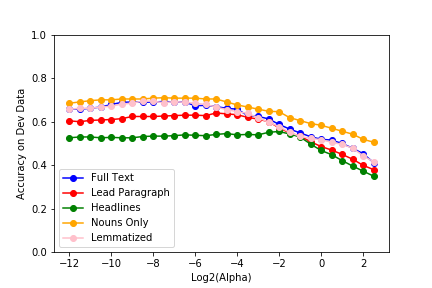
\includegraphics[scale=0.55]{mnb_accuracy}
\caption{MNB Accuracy on Dev Data}
\label{fig:mnb-acc}
\end{figure}

\begin{figure}
\centering
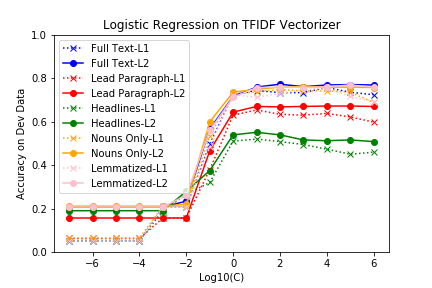
\includegraphics[scale=0.55]{lr_accuracy}
\caption{LR Accuracy on Dev Data}
\label{fig:lr-acc}
\end{figure}

\begin{table}
\centering
%\small
\resizebox{\columnwidth}{!}{
\begin{tabular}{lrrr}
	\toprule
	\textbf{Model Input} & \textbf{Vocabulary} & \textbf{90\% Length} & \textbf{Padding} \\
	\midrule
	Full Text			& 129,165	& 1,225	& 500 \\
	Lead Paragraph	& 63,733	& 135	& 135 \\
	Headlines			& 19,724	& 10		&10 \\
	Nouns			& 97,557	& 374	& 374 \\
	Lemmas			& 113,923	& 1,239	& 500 \\
	\bottomrule
\end{tabular}
}
\caption{CNN Vocabulary and Padding Sizes}
\label{tbl:cnn}
\end{table}

\section{Results \& Discussion}
\label{sec:results}

Note: \cite{Wermter:02} uses only top 8 topics.

\begin{table}
\centering
%\small
\resizebox{\columnwidth}{!}{
\begin{tabular}{lrrrc}
	\toprule
	& \multicolumn{3}{c}{\textbf{Model Type}} & \\
	\cmidrule{2-4}
	\textbf{Model Input} & \textbf{MNB} & \textbf{LR} & \textbf{CNN} & \multicolumn{1}{c}{\textbf{Best Model}} \\
	\midrule
	Full Text			& \textbf{0.}	& \textbf{0.}	& 0.		& \cellcolor[gray]{0.92} X \\
	Lead Paragraph	& 0.		& 0.		& \textbf{0.}	& \cellcolor[gray]{0.92} X \\
	Headlines			& 0.		& 0.		& 0.		& \cellcolor[gray]{0.92} X \\
	Nouns			& 0.		& 0.		& 0.		& \cellcolor[gray]{0.92} X \\
	Lemmas			& 0.		& 0.		& 0.		& \cellcolor[gray]{0.92} X \\
	\midrule
	\multirow{2}{*}{\textbf{Best Input}} & \cellcolor[gray]{0.92} X & \cellcolor[gray]{0.92} X & \cellcolor[gray]{0.92} X & \cellcolor[gray]{0.75} \textbf{X} \\
	& \cellcolor[gray]{0.92} X & \cellcolor[gray]{0.92} X & \cellcolor[gray]{0.92} X & \cellcolor[gray]{0.75} \textbf{in X} \\
	\bottomrule
\end{tabular}
}
\caption{Accuracies on Test Data}
\label{tbl:acc}
\end{table}

\begin{table}
\centering
%\small
\resizebox{\columnwidth}{!}{
\begin{tabular}{lrrrc}
	\toprule
	& \multicolumn{3}{c}{\textbf{Model Type}} & \\
	\cmidrule{2-4}
	\textbf{Model Input} & \textbf{MNB} & \textbf{LR} & \textbf{CNN} & \multicolumn{1}{c}{\textbf{Best Model}} \\
	\midrule
	Full Text			& \textbf{0.}	& \textbf{0.}	& 0.		& \cellcolor[gray]{0.92} X \\
	Lead Paragraph	& 0.		& 0.		& \textbf{0.}	& \cellcolor[gray]{0.92} X \\
	Headlines			& 0.		& 0.		& 0.		& \cellcolor[gray]{0.92} X \\
	Nouns			& 0.		& 0.		& 0.		& \cellcolor[gray]{0.92} X \\
	Lemmas			& 0.		& 0.		& 0.		& \cellcolor[gray]{0.92} X \\
	\midrule
	\multirow{2}{*}{\textbf{Best Input}} & \cellcolor[gray]{0.92} X & \cellcolor[gray]{0.92} X & \cellcolor[gray]{0.92} X & \cellcolor[gray]{0.75} \textbf{X} \\
	& \cellcolor[gray]{0.92} X & \cellcolor[gray]{0.92} X & \cellcolor[gray]{0.92} X & \cellcolor[gray]{0.75} \textbf{in X} \\
	\bottomrule
\end{tabular}
}
\caption{Weighted F1 Scores on Test Data}
\label{tbl:f1}
\end{table}

\section{Conclusion}
\label{sec:conc}

No time for: SVM, gradient boosted trees

An interesting future project would be to run an unsupervised topic classification algorithm on this corpus (e.g. \citeauthor{Martin:15}~\shortcite{Martin:15} use the Latent Dirichlet Allocation algorithm) and compare those results to the supervised learning results.

\bibliography{final-report} % references .bib file
\bibliographystyle{acl_natbib} % references acl_natbib.bst

\end{document}
